\subsection{Simulation of the Filter}
The performance of the Kalman filter is tested through simulations. These are performed by applying some arbitrary inputs to the model of the system derived in \autoref{chap:model}. The signals obtained are transformed into measurements by adding noise whose variance is the present in the physical sensors and shown in \autoref{app:IMUVariances}. The simulations are also used to tune the filters so a good estimation of the states is obtained. The tuning parameters are the elements in the covariance matrix for the states, $\vec{Q}_\mathrm{att}$. 

The procedure starts by focusing on the estimation of the angular velocities and the angular accelerations as these states are mostly dependent on the measurement given by the gyroscope and act as input for the attitude state estimation.

The result is shown in \autoref{fig:sim_yawdot} and \ref{fig:sim_yawddot}, where the estimations for $\dot{\psi}$ and $\ddot{\psi}$ are plotted. As it can be seen, both signals are correctly estimated. It is especially remarkable in $\ddot{\psi}$, as there are no direct measurements for this state.
\begin{figure}[H]
	\captionbox 
	{   
		Result of the estimation of the angular velocity around $z_\mathrm{b}$, compared to the real value in the simulation and the measurements.
		\label{fig:sim_yawdot}
	}                                                        
	{  
		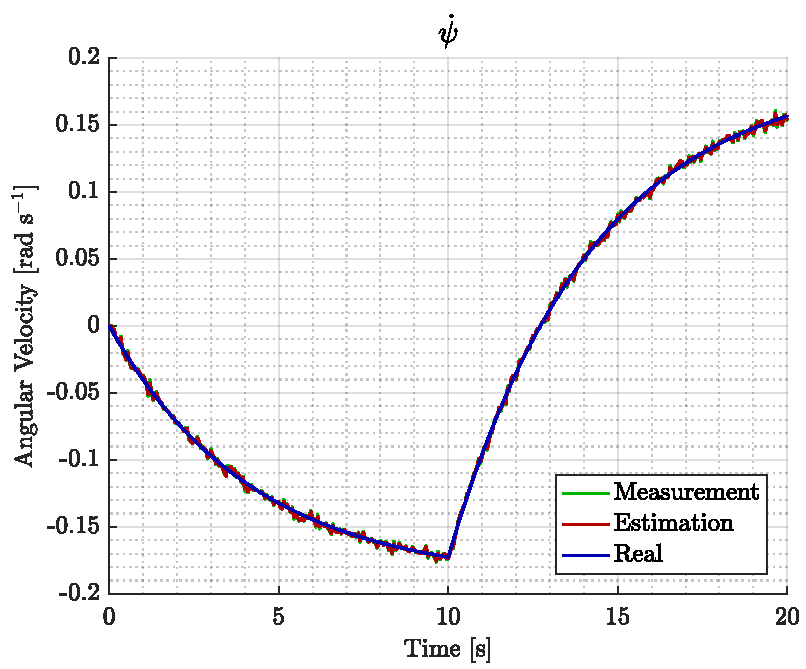
\includegraphics[width=.45\textwidth]{figures/sim_yawdot}         
	}        
	\hspace{5pt}                 
	\captionbox  
	{      
		Estimation of the angular acceleration around $z_\mathrm{b}$, compared to the real value.
		\label{fig:sim_yawddot}
	}                                                        
	{
		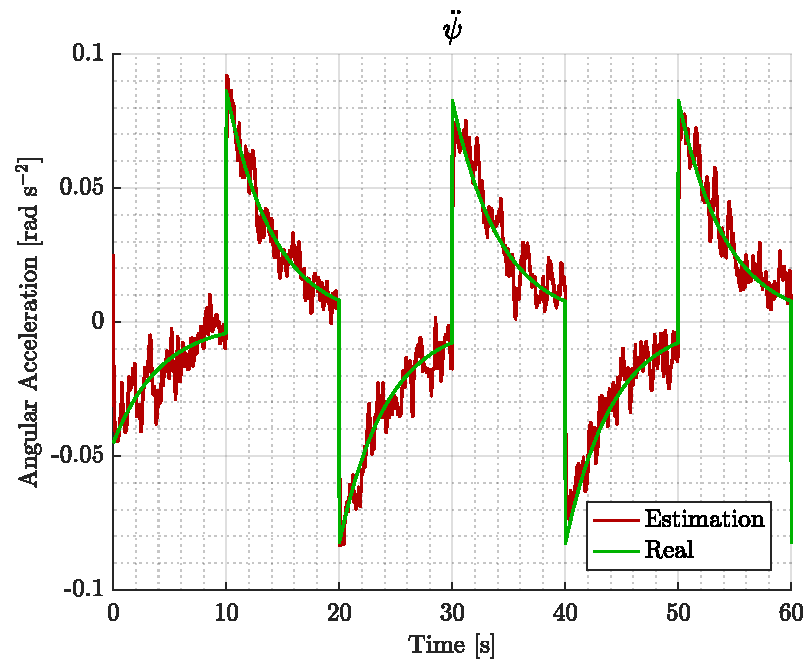
\includegraphics[width=.45\textwidth]{figures/sim_yawddot}
	}
\end{figure}

\autoref{fig:sim_yaw} shows the estimation of the heading, $\psi$ as an example of the attitude estimation of the Kalman filter. This plot is obtained with the final values for the state covariance matrix elements.
\begin{figure}[H]
    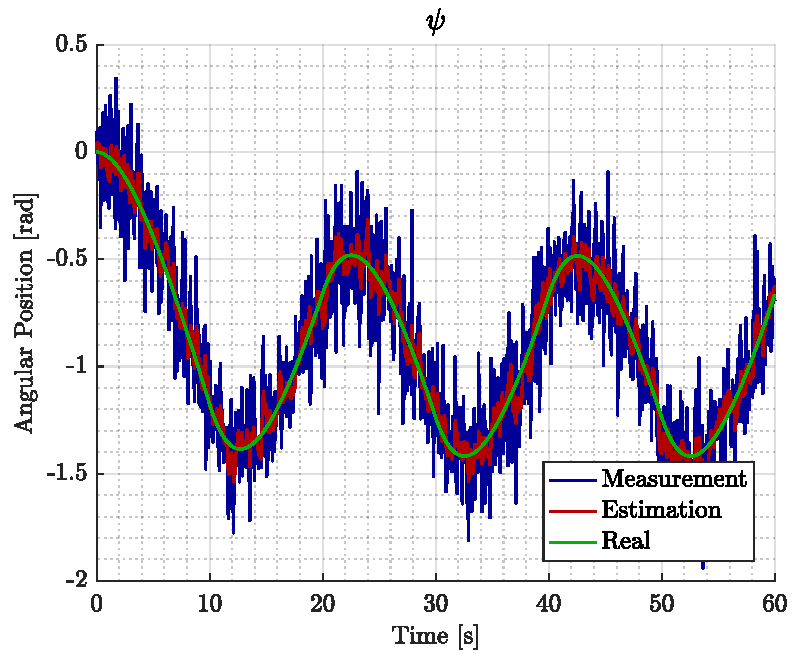
\includegraphics[width=0.5\textwidth]{figures/sim_yaw}
    \caption{Result of the estimation of the heading, compared to the real value in the simulation and the measurements.}
    \label{fig:sim_yaw}
\end{figure}
In this case, the filter is also able to remove most of the noise present in the measurement and provide an estimation close to the real value. 

The final values obtained for $\vec{Q}_\mathrm{att}$ are
\begin{flalign}
	\vec{Q}_\mathrm{att} &= diag\left(10^{-5},10^{-5},10^{-5},10^{-4},10^{-4},10^{-10},10^{-2},10^{-2},10^{-2} \right) \ .
\end{flalign}
